% BHU PYQ -- Professional Exam Template
\documentclass[11pt,a4paper]{article}

\usepackage[a4paper,top=2.5cm,bottom=2.5cm,left=2.8cm,right=2.8cm,headheight=14pt]{geometry}
\usepackage{amsmath,amssymb}
\usepackage[T1]{fontenc}
\usepackage[utf8]{inputenc}
\usepackage{lmodern}
\usepackage{microtype}
\usepackage{fancyhdr}
\usepackage{enumitem}
\usepackage{hyperref}
\usepackage{lastpage}
\usepackage{parskip}
\usepackage{tikz}
\usetikzlibrary{arrows.meta,shapes,positioning,decorations.pathreplacing}

\hypersetup{colorlinks=true,urlcolor=black,linkcolor=black,
  pdftitle={B.Sc. (Hons.) Zoology Sem-VI ZOB-605 -- BHU PYQ}}

\pagestyle{fancy}
\fancyhf{}
\renewcommand{\headrulewidth}{0.4pt}
\renewcommand{\footrulewidth}{0.4pt}
\fancyhead[L]{\small   \textit{Banaras Hindu University}}
\fancyhead[R]{\small   \textit{Zoology Paper: ZOB-605}}
\fancyfoot[C]{\small Page  \thepage\ of \pageref{LastPage}}


\newlist{parts}{enumerate}{2}
\setlist[parts,1]{label=(\alph*),leftmargin=*,itemsep=4pt,topsep=3pt}
\setlist[parts,2]{label=(\roman*),leftmargin=*,itemsep=2pt,topsep=2pt}

\newcommand{\pts}[1]{\hfill   \textit{[#1]}}


\begin{document}


\begin{center}
  {\large\bfseries BANARAS HINDU UNIVERSITY}\\[2pt]
  {\normalsize B.Sc. (Hons.) Semester VI Examination, 2022-23}\\[6pt]
  \rule{0.8\linewidth}{0.5pt}\\[6pt]
  {\large\bfseries Zoology}\\[4pt]
  {\large\bfseries Paper: ZOB-605 --- Immunology and Parasitology}\\[4pt]
  {\normalsize Time: Three hours \hfill Full Marks: 70}
\end{center}

\rule{\linewidth}{0.4pt}

\smallskip



\noindent   \textit{Note: Answer three questions from Section-A (including Question No. 1 which is compulsory) and three questions from Section-B (including Question No. 1 which is compulsory). Use a separate answer book for each section. The figures in the right-hand margin indicate marks.}

\bigskip

\begin{center}
   \textbf{SECTION -- A} \\
   \textbf{(Immunology) (Marks: 35)}
\end{center}




\noindent   \textbf{Question 1.} Answer the following parts:

\begin{parts}
  \item State whether the following statements are True or False. Justify your answer in 2--3 sentences each:\pts{$4  \times 2 = 8$}
  
\begin{parts}
    \item Type II hypersensitivity is mediated by immune complex.
    \item B-cell epitopes are always presented with MHC.
    \item Herd immunity is achieved in highly contagious disease when 40\% of population is vaccinated.
    \item Graves' disease affects the thyroid gland.
  \end{parts}
  
  \item Define the following:\pts{$3  \times 1 = 3$}
  
\begin{parts}
    \item M cells
    \item Immunodeficiency
    \item Adaptive immunity.
  \end{parts}
\end{parts}

\medskip


\noindent   \textbf{Question 2.} Describe the mechanism of antigen processing and presentation via MHC class I and class II to T lymphocytes.\pts{12}

\pagebreak

\medskip


\noindent   \textbf{Question 3.} Answer the following:

\begin{parts}
  \item Discuss the properties of an ideal vaccine.\pts{5}
  \item Discuss the structure of immunoglobulin and describe the function of IgG, IgA and IgM.\pts{7}
\end{parts}


\begin{center}

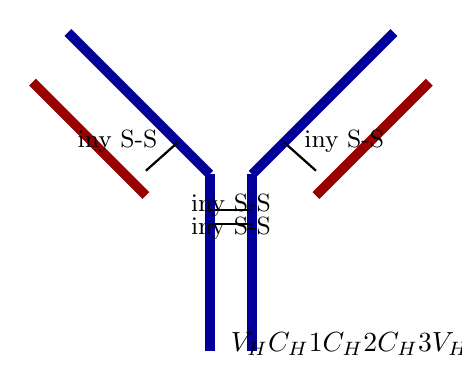
\begin{tikzpicture}[scale=0.9, >=Stealth, every node/.style={font=\small}]
  % Define colors
  \colorlet{heavycol}{blue!60!black}
  \colorlet{lightcol}{red!60!black}
  
  % Left heavy chain
  \draw[line width=3.5pt, heavycol] (-0.3, 0) -- (-0.3, 2.5);
  \draw[line width=3.5pt, heavycol] (-0.3, 2.5) -- (-2.3, 4.5);
  
  % Right heavy chain
  \draw[line width=3.5pt, heavycol] (0.3, 0) -- (0.3, 2.5);
  \draw[line width=3.5pt, heavycol] (0.3, 2.5) -- (2.3, 4.5);
  
  % Left light chain
  \draw[line width=3.5pt, lightcol] (-1.2, 2.2) -- (-2.8, 3.8);
  
  % Right light chain
  \draw[line width=3.5pt, lightcol] (1.2, 2.2) -- (2.8, 3.8);
  
  % Disulfide bonds (hinge)
  \draw[thick, black] (-0.3, 1.8) -- (0.3, 1.8) node[midway, above=-1pt] { iny S-S};
  \draw[thick, black] (-0.3, 2.0) -- (0.3, 2.0) node[midway, below=-1pt] { iny S-S};
  
  % Disulfide bonds (H-L)
  \draw[thick, black] (-0.75, 2.95) -- (-1.2, 2.55) node[midway, above left=-3pt] { iny S-S};
  \draw[thick, black] (0.75, 2.95) -- (1.2, 2.55) node[midway, above right=-3pt] { iny S-S};
  
  % Labels
  
ode[left, heavycol] at (-0.5, 1.2) {Heavy Chain};
  
ode[right, lightcol] at (2.0, 2.4) {Light Chain};
  
  % Domains
  
ode[draw, fill=blue!10, rounded corners=2pt, minimum width=0.6cm, minimum height=0.4cm, rotate=45] at (-1.8, 4.0) {$V_H$};
  
ode[draw, fill=blue!10, rounded corners=2pt, minimum width=0.6cm, minimum height=0.4cm, rotate=45] at (-1.1, 3.3) {$C_H1$};
  
ode[draw, fill=blue!10, rounded corners=2pt, minimum width=0.4cm, minimum height=0.6cm] at (-0.3, 1.4) {$C_H2$};
  
ode[draw, fill=blue!10, rounded corners=2pt, minimum width=0.4cm, minimum height=0.6cm] at (-0.3, 0.6) {$C_H3$};

  
ode[draw, fill=blue!10, rounded corners=2pt, minimum width=0.6cm, minimum height=0.4cm, rotate=-45] at (1.8, 4.0) {$V_H$};
  
ode[draw, fill=blue!10, rounded corners=2pt, minimum width=0.6cm, minimum height=0.4cm, rotate=-45] at (1.1, 3.3) {$C_H1$};
  
ode[draw, fill=blue!10, rounded corners=2pt, minimum width=0.4cm, minimum height=0.6cm] at (0.3, 1.4) {$C_H2$};
  
ode[draw, fill=blue!10, rounded corners=2pt, minimum width=0.4cm, minimum height=0.6cm] at (0.3, 0.6) {$C_H3$};

  
ode[draw, fill=red!10, rounded corners=2pt, minimum width=0.6cm, minimum height=0.4cm, rotate=45] at (-2.3, 3.3) {$V_L$};
  
ode[draw, fill=red!10, rounded corners=2pt, minimum width=0.6cm, minimum height=0.4cm, rotate=45] at (-1.6, 2.6) {$C_L$};

  
ode[draw, fill=red!10, rounded corners=2pt, minimum width=0.6cm, minimum height=0.4cm, rotate=-45] at (2.3, 3.3) {$V_L$};
  
ode[draw, fill=red!10, rounded corners=2pt, minimum width=0.6cm, minimum height=0.4cm, rotate=-45] at (1.6, 2.6) {$C_L$};
  
  % Labels
  
ode[above] at (-2.3, 4.5) {Antigen-binding site};
  
ode[above] at (2.3, 4.5) {Antigen-binding site};
  
  
ode[font=\bfseries] at (0, -0.6) {Structure of Immunoglobulin G (IgG)};
\end{tikzpicture}
\end{center}

\medskip


\noindent   \textbf{Question 4.} Write short notes on the following:\pts{$3  \times 4 = 12$}

\begin{parts}
  \item Lymphocytes
  \item Hapten
  \item Spleen.
\end{parts}

\bigskip

\begin{center}
   \textbf{SECTION -- B} \\
   \textbf{(Parasitology) (Marks: 35)}
\end{center}




\noindent   \textbf{Question 1.} Answer the following parts:

\begin{parts}
  \item State whether the following statements are True or False. Justify your answer in 2--3 sentences each:\pts{$2  \times 2 = 4$}
  
\begin{parts}
    \item Individual suffering from trichinosis develops myositis, fever, periorbital oedema within a week.
    \item Unembryonated eggs of   \textit{Paragonimus westermani} are coughed up and voided in sputum.
  \end{parts}
  
  \item Differentiate between the following:\pts{$2  \times 2 = 4$}
  
\begin{parts}
    \item Endotoxin and Exotoxin
    \item Tachyzoite and Bradyzoite.
  \end{parts}
  
  \item Define the following:\pts{$3  \times 1 = 3$}
  
\begin{parts}
    \item Hyperparasites
    \item Paratenic host
    \item Zooanthroponosis.
  \end{parts}
\end{parts}

\pagebreak

\medskip


\noindent   \textbf{Question 2.} Discuss the asexual cycle of   \textit{Plasmodium vivax}. Comment on the clinical manifestations and control measures of the disease.\pts{12}


\begin{center}

\begin{tikzpicture}[scale=0.85, >=Stealth, every node/.style={font=\small}]
  % Define stages as nodes
  
ode[draw, rounded corners, fill=green!10, align=center] (sporo) at (0, 4) {Sporozoites \\ (Injected by Mosquito)};
  
ode[draw, rounded corners, fill=orange!10, align=center] (liver) at (3.8, 2.5) {Invasion of Liver Cell \\ (Exo-erythrocytic cycle)};
  
ode[draw, rounded corners, fill=orange!15, align=center] (schiz1) at (4.8, 0) {Liver Schizont \\ \& Merozoites};
  
ode[draw, rounded corners, fill=red!10, align=center] (rbc) at (2.5, -2.5) {Invasion of RBC \\ (Erythrocytic cycle)};
  
ode[draw, rounded corners, fill=red!15, align=center] (ring) at (0, -4) {Ring Stage \\ (Trophozoite)};
  
ode[draw, rounded corners, fill=red!20, align=center] (schiz2) at (-2.5, -2.5) {Erythrocytic Schizont \\ (Merozoite release)};
  
ode[draw, rounded corners, fill=purple!10, align=center] (gam) at (-4.8, 0) {Gametocytes \\ (Infective to Mosquito)};
  
  % Draw arrows
  \draw[->, ultra thick, blue!60!black] (sporo) to[out=0, in=120] (liver);
  \draw[->, ultra thick, blue!60!black] (liver) to[out=-30, in=90] (schiz1);
  \draw[->, ultra thick, blue!60!black] (schiz1) to[out=210, in=30] (rbc);
  \draw[->, ultra thick, red!60!black] (rbc) to[out=240, in=0] (ring);
  \draw[->, ultra thick, red!60!black] (ring) to[out=180, in=-60] (schiz2);
  \draw[->, ultra thick, red!60!black] (schiz2) to[out=30, in=150] (rbc); % Cycle back
  \draw[->, ultra thick, purple!60!black] (schiz2) to[out=120, in=-90] (gam);
  \draw[->, ultra thick, green!60!black] (gam) to[out=90, in=180] (sporo);
  
  % Labels
  
ode[above, font=\bfseries] at (0, 4.8) {Asexual Life Cycle of   \textit{Plasmodium vivax}};
\end{tikzpicture}
\end{center}

\medskip


\noindent   \textbf{Question 3.} Describe the life cycle and pathogenesis of   \textit{Diphyllobothrium latum}. Briefly discuss its treatment and prophylactic measures.\pts{12}

\medskip


\noindent   \textbf{Question 4.} Write notes on the following:\pts{$2  \times 6 = 12$}

\begin{parts}
  \item Host-parasite coevolution
  \item Intestinal amoebiasis.
\end{parts}

\vfill
\rule{\linewidth}{0.4pt}

\begin{center}\small
\href{https://bhu-exam.vercel.app/}{Click Here}\\[4pt]\href{https://me-aryan.vercel.app/}{Click Here}\\[4pt]\href{https://quashan-me.vercel.app/}{Click Here}
\end{center}

\end{document}
